%!TEX root = main.tex
\chapter{Expert Review}
\section{Overview}
The expert evaluation was with a senior scientist at Sintef Information and Communication Technology\footnote{Sintef ICT: \url{http://www.sintef.no/home/Information-and-Communication-Technology-ICT/}}, which also works as adjunct associate professor at NTNU. The evaluator is an expert in the field of agile software development and knowledge management in software companies. The evaluator has published several case studies of agile teamwork in the industry. He also had knowledge of GitHub and the use of it in agile development teams.  Apart from the expert review, the evaluator was never directly involved in our thesis.  \\
The evaluation performed was a type of expert walkthrough as described in \emph{Interaction Design - Beyond Human Computer Interaction}\cite{rogers2011interaction}. The evaluation we performed differs in that we also evaluate how the application can support agile software development teams and reflection through revisiting experiences. We presented the main features of the application and proceeded with a walkthrough of the application in its production state. The walkthrough consisted of typical tasks in our scenarios. After the walkthrough we had an open discussion with the evaluator on possible shortcomings or limitations, and also any advantages the evaluator had identified. We asked the evaluator to present his ideas on how our application could improve reflection in agile software development teams. We wanted an objective evaluation so we did not initially present any of our own thoughts about the application and its goals. \\
The evaluator suggested several possible limitations in the application, and also commented on how our application met some of the problems that often arise in development teams and how he could see our application potentially help limit these problems. We particularly went through the reflection workshop questions[ref her], to get feedback on the feasability of these and triggering reflection in a retrospective session. 
In addition to advantages and limitations of our applications the evaluator had some input towards related work he had seen, and how we could conduct the final evaluation in the best way. This included possible questions to ask, how to get the best possible output from the evaluation group and also some theory on how to analyze the results we got. \\
The feedback we got from the expert showed that we had proposed solutions to many of the problems he had encountered through his studies of agile teams, and specifically how to trigger better reflection. The evaluator also had some valuable feedback on possible shortcomings we had not thought of, that is an issue in a day to day working environment. 

\subsection{Overall Feedback}
The evaluation with the Sintef expert left us with the impression that the evaluator was satisified with the general functionality of the application, in terms of agile teams and reflection in these teams. 
At the point of evaluation, the application had been deployed to production state, and so most of the functionality was in place. The evaluator stated that the choices we had made on the data collection and representation of these was satisfying, as it allowed and encouraged users to reflect on their experiences, while not being too intrusive on the daily work routine. Both in aspects of individual and collaborative reflection the application and its functionality was satisfactory. As for the team aspect the evaluator saw a limitation in that it was generally hard to get new tools into the daily routine of developers. Especially the way we expect users to use \# \emph{hashtags} to tag important elements in the commit message, might take some time to work in. The evaluator expressed that he was happy with the design choices made and that we chose a web-application as a platform. This way the application is available for all individuals in the team, on a wide variety of devices. This availability is important in order to furhter lower the threshold of usage. Apart from general feedback and app-specific feedback we also got some feedback regarding the final evaluation we conducted. Especially what questions to ask, compare their previous retrospectives routines with a retrospective using our app in beforehand. Also feedback on how to properly analyze the results we would get was valuable, as the evaluator had experience in his studies, that showed possible reasons for why a specific outcome could occur. 

\subsection{App-specific feedback}
Here we will present the challenges the evaluator presented in the aspect of teamwork and reflection in agile software development teams. We will then detail the feedback from the evaluator on how potentially the PeacefulBanana application can answer these challenges. 
\subsubsection{Challenges}
\begin{figure}[h!]
    \centering
        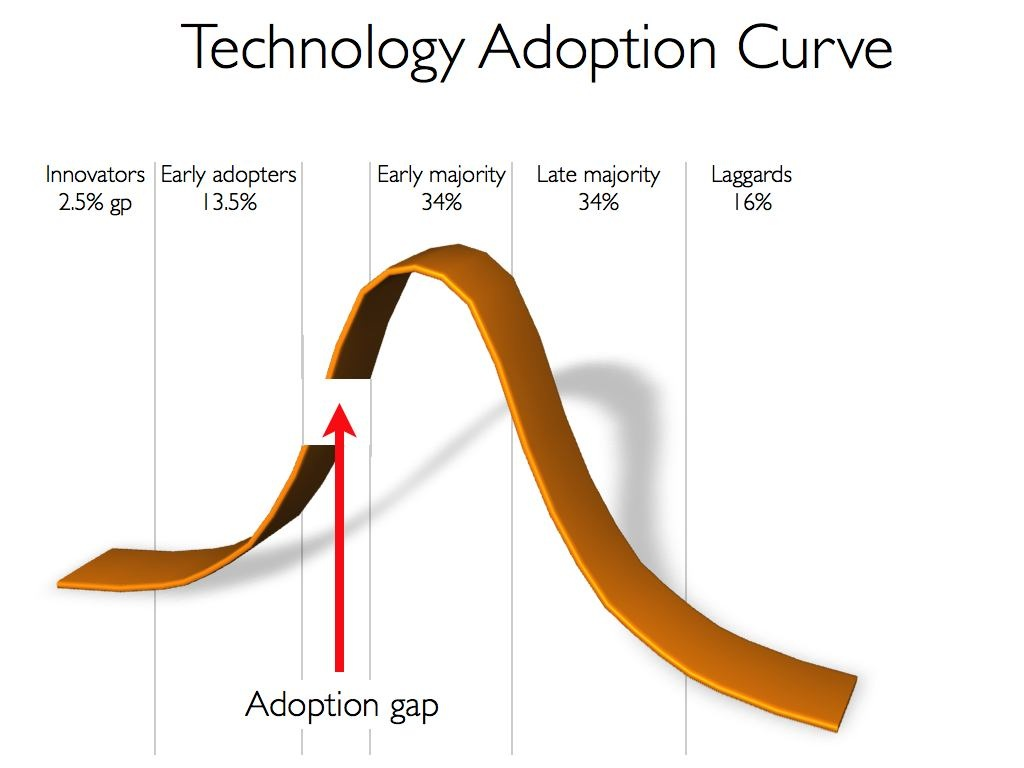
\includegraphics[width=\textwidth]{rogerscurve}
    \caption{Roger's Innovation Adoption Curve}
    \label{rogerscurve}
\end{figure}

\begin{itemize}
	\item Non-intrusive application: The threshold of integrating new tools into the routines of software developers is hard. The evaluator specifically referred to the \emph{Technology Adoption Curve} presented by Rogers\cite{rogers2010diffusion}, which refers to the chasm between innovators or early adopters and the early majority. This curve can be seen in Figure \ref{rogerscurve}.
	\item Uniqueness: The application should meet a demand which hasn't already been met. Also the application should provide something that a normal retrospective does not.
	\item Agile integration: How can the application be integrated into an agile environment, helping the team to be agile and not removing the agililty from the team. 
	\item Memories change over time: Memories are dynamic and change over time, so there can be a lack of memorizing all important situations in a retrospective. 
	\item Priorities: Often agile teams develop what the developers are motivated for, and not what the customer prioritizes highest. These wrong-placed priorities can be hard to pick up. 
	\item Competence-overlap: Agile teams are most efficient and deliver the highest quality work when atleast two people have the same competence, so that one can ask for help and code can be reviewed by a peer. When a developer is left alone on a piece of work, integrating these parts with the rest of the project can be an issue.
	\item Re-work: Re-doing the same piece of work is also a challenge development teams can meet. When developers constantly revisits work that already has been accepted, to make unnecessary changes, the progress of the project is slowed down. Detection of this can allow for a discussion and allowing the team to progress.
	\item Level of expertise: Developers often have different levels of expertise, and different areas of expertise. Even though a developer have a high amount of impact on the code-lines commited to a project, this does not mean the others don't do important work. 
\end{itemize}

\subsubsection{Features}
The evaluator had some input to what additional functionality that might be implemented: 
\begin{itemize}
	\item Show parts of the source-code in the PeacefulBanana application, creating a sort of \emph{What is new?} functionality to the team. 
	\item Integrate a burndown-chart into the application. 
\end{itemize}

%  Keeping the required involvement by users of the application to a minimum was a good design choice, 
% # Feedback fra Torgeir:
% * Stille alternativer opp mot hverandre i rapporten, f.eks om de ser en nytte versus å kun bruke github. 
% * Belyser appen nye ting i forhold til vanlige retrospektiver?
% * Spørre gruppa hva de gjorde på tidligere retrospektiver, og om bruken av appen kan hjelpe. Spør de som ikke har deltatt at dersom de hadde brukt tags osv. hadde de sett nytten? Og da evt til hvilken grad.  
% * Spør: Hvorfor har de ikke brukt det? Tid? Features? Vanskelig? Var det i veien?

% ## Fordeler
% * Non-intrusive: Veldig bra
% * Er unikt: Han hadde ikke sett noe lignende verktøy
% * Er et kjent problem at man ikke husker alt, notes kan hjelpe men det kan bli mye data å analysere som går litt imot smidig. Viktig spørsmål å se om man husker mer ved bruk av appen, altså om man går glipp av noe uten å bruke appen. 
%* Finne feilprioriteringer, ofte er det feilvurderinger av hva som er viktig å gjøre. Oftest gjøres det som utviklerne vil og ikke kunden. Med appen kan man se tendenser til mye jobbing på feil ting. Samt. at man ser at milestones går overdue. 
%* Koble ting opp mot teorimodell: Kompetanseoverlapp. Sitter noen mye alene? Tagclouden kan vise slike tendenser.
%* Re-work: Oppdage dette, vi har muligheter til å oppdage mye gjenåpninger på issues og forklare dette. Mye jobbing med samme ting kan oppdages i appen. 

%## Utfordringer
%* Får man noe nyttig utav det
%* Få personer til å faktisk bruke tags i hverdagen. 
%* Generelt vanskelig terskel å få folk til å bruke verktøy. -> Rogers curve-diagram. 
%* Det vil være folk som ikke vil bidra like mye, early adopters vs laggers. 
%* Forskjellig nivå på utviklere. Noen vil dominere commit statistikken, men betyr det da at de er viktigere enn de andre? (Som kanskje gjør andre viktige ting i prosjektet). Det kan gi feil totalbilde. 

%## Features
%* Ha deler av kildekoden i peaceful, en slags "hva har skjedd" feature. Overlapper litt med github
%* Burndown chart. Har github noe lignende kanskje? sjekk

%## Studier
%* Vitner husker ofte feil i rettsaker -> hukommelse er ikke bombesikker/til å stole på alltid. Derfor lurt å ta ferske erfaringer

%### Related Work:
%* Hackystat : https://code.google.com/p/hackystat/